\documentclass[tikz,border=8pt]{standalone}
\usepackage{amsmath}
\begin{document}
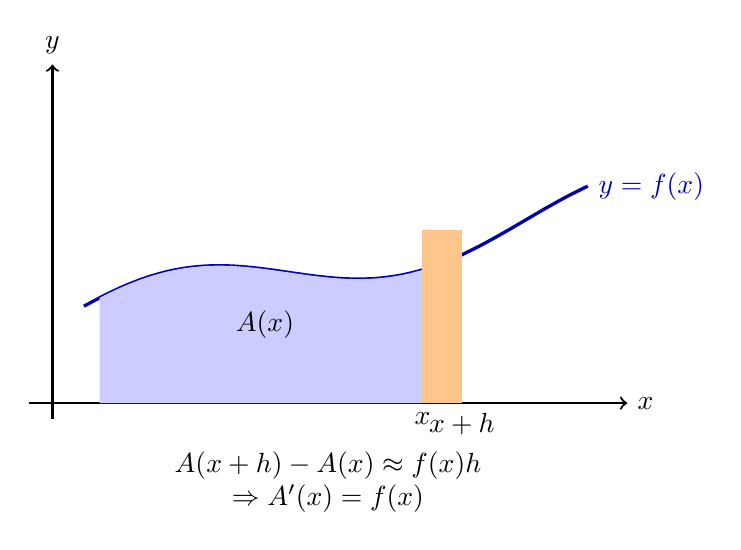
\begin{tikzpicture}
\draw[->,thick] (-0.3,0)--(7.3,0) node[right] {$x$};
\draw[->,thick] (0,-0.2)--(0,4.3) node[above] {$y$};
\draw[very thick,blue!70!black] plot[smooth,domain=.4:6.8] (\x,{1+0.35*sin(60*\x)+0.22*\x}) node[right] {$y=f(x)$};
\fill[blue!20] (.6,0)--plot[smooth,domain=.6:4.7] (\x,{1+0.35*sin(60*\x)+0.22*\x})--(4.7,0)--cycle;
\fill[orange!45] (4.7,0) rectangle (5.2,2.2);
\node[below] at (4.7,0) {$x$}; \node[below] at (5.2,0) {$x+h$};
\node at (2.7,1) {$A(x)$};
\node[align=center] at (3.5,-1) {$A(x+h)-A(x)\approx f(x)h$\\$\Rightarrow A'(x)=f(x)$};
\end{tikzpicture}
\end{document}